\section{Methods}
The framework calculates burnt area based on the maximum allowed burnt area from limitations imposed by four controls: fuel, moisture, ignition, and anthropogenic suppression. These controls are described from remote sensed and meteorological observations. Parameters relating controls to fire are optimised against Global Fire Emissions Database (GFED4s) burnt area observations \citep{Giglio2013}.
The framework could probably be used on a range of temporal and spatial resolutions
\hlb{(scale dependency might be something to test in the future?)}.
Here, burnt area is calculated monthly on a 0.5$^{\circ}$ CRUTS3.22 grid \citep{harris2014cru}, between Jan 2000 and Dec 2010 (the period of data overlap).

%%%%%%%%%%%%%%%%%%%%%%%%%%%%%%%%%%%%%%%%%%%%%%%%%%%%%%%%%%%%%%%%%%%%%%%%%%%%%%%%%%%%%%%%%
%% Overview                                                                            %%
%%%%%%%%%%%%%%%%%%%%%%%%%%%%%%%%%%%%%%%%%%%%%%%%%%%%%%%%%%%%%%%%%%%%%%%%%%%%%%%%%%%%%%%%%
\subsection{Overview}

The framework assumes that 100\% burnt area occurs in perfect fire conditions,  i.e. complete fuel coverage, no moisture, saturated ignition and no agricultural or urban fragmentation. This is analogous to the dry season in tropical savanna and grasslands \citep{kelley2014modelling}, particularly parts of Northern Australia \citep{murphy2013fire} and the Sahel \citep{van2008climate} which experience complete buring each year.
Burnt area is reduced as each control becomes sub-optimal, i.e.
    fuel loads become discontinuous  (e.g. desert areas)
    or too moist (e.g. Humid evergreen forests),
    if there is a lack of ignition (shown to influence interannual variability in parts Southern Australia \cite{bradstock2010biogeographic} \hlb{and probably some other places}),
    or with increased human influence on the landscape (e.g. cropland or urban areas).
Fractional burnt area ($F$) is the product of the maximum allowed burnt area for each control ($F_i$).
\begin{equation}
    F=\Pi_{i} F_i
    \label{equ:LimFIRE}
\end{equation}
\hlb{Is it widley known that $\Pi$ means product?}

A controls maximum burnt area is related to fuel loads, moisture, ignitions or suppression via the logistic function, as per \citet{bistinas2014causal}:

\begin{equation}
    f(x) = 1 / (1 + e^{-k \cdot (x - x_0)})
    \label{equ:fx}
\end{equation}
where $k$ described the steepness of the curve and $x_0$ is the curves midpoint (see figure ~\ref{fig:Logistic_fun}).

\begin{figure}[!ht]
  \centering
    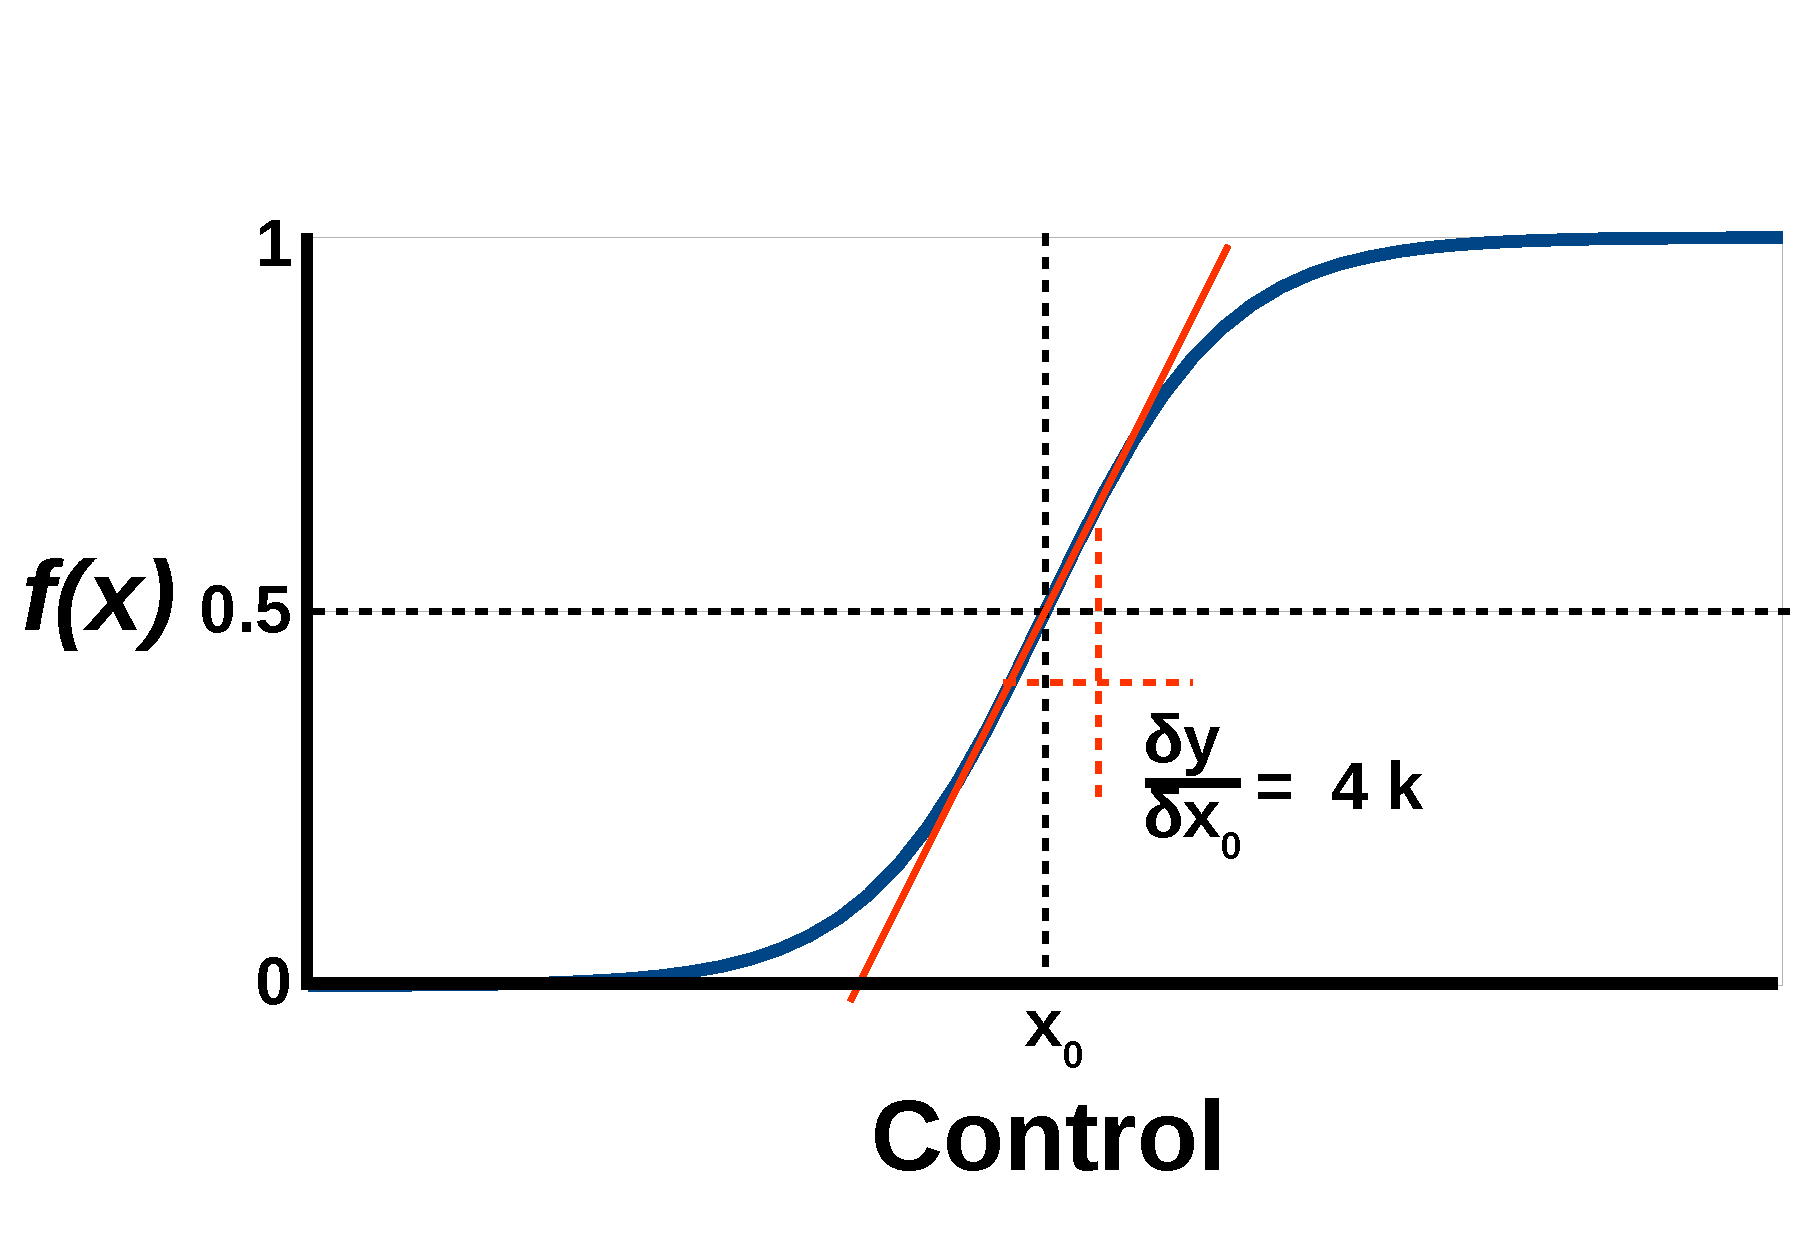
\includegraphics[width=0.67\textwidth]{diagrams/Logistic_fun.pdf}
  \caption{Logistic function.}
  \label{fig:Logistic_fun}
\end{figure}

Fire increases with increasing fuel load ($F_w$) and igntions ($F_{ig}$), and decreases with moisture ($F_{\omega}$) and anthropagenic supression ($F_s$). Therefore:

\begin{equation}
    \begin{split}
        F_{w} = f(w) \\
        F_{\omega} = 1 - f(\omega) \\
        F_{ig} = f(ig) \\
        F_{s} = 1- f(s)
    \end{split}
    \label{equ:LimFIRE.x}
\end{equation}

\begin{figure}[!ht]
  \centering
    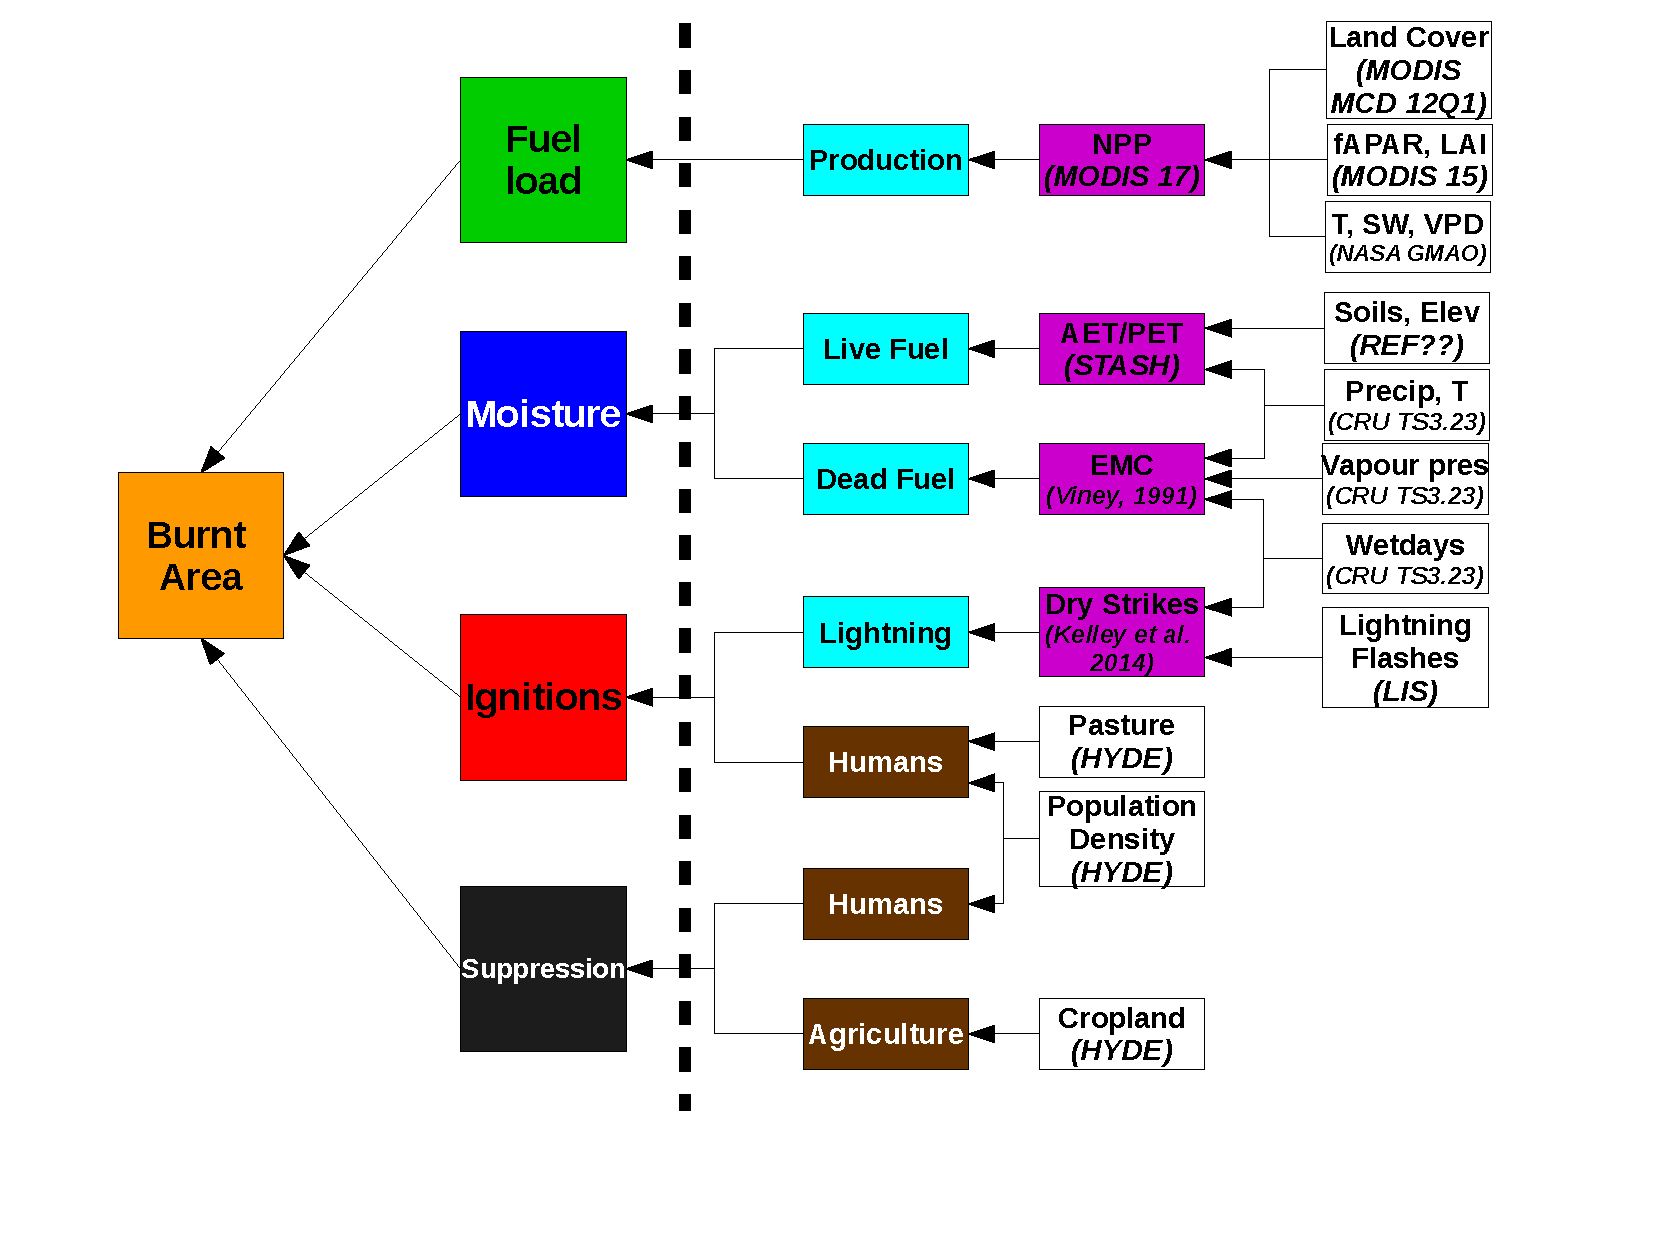
\includegraphics[width=0.8\textwidth]{diagrams/Model_schematic.pdf}
  \caption{Framework description.}
\end{figure}


\subsection{Inputs}

\colorlet{shadecolor}{Mycolor3}
\begin{shaded}
\subsubsection{Fuel ($w$)}
The framework will use a measure of fractional cover as a proxy for fuel continuity (i.e, annual mean or maximum fAPAR, as used by \citet{knorr2014impact,knorr2016climate} or MODIS fractional cover). \citet{bistinas2014causal} uses SeaWiFs fAPAR, but this product was discontinued in 2005, so would reduce our comparison period. Other fAPAR/Fractional cover products would probably cover a larger period.
\end{shaded}
\colorlet{shadecolor}{Mycolor2}

\begin{figure}[!ht]
  \centering
    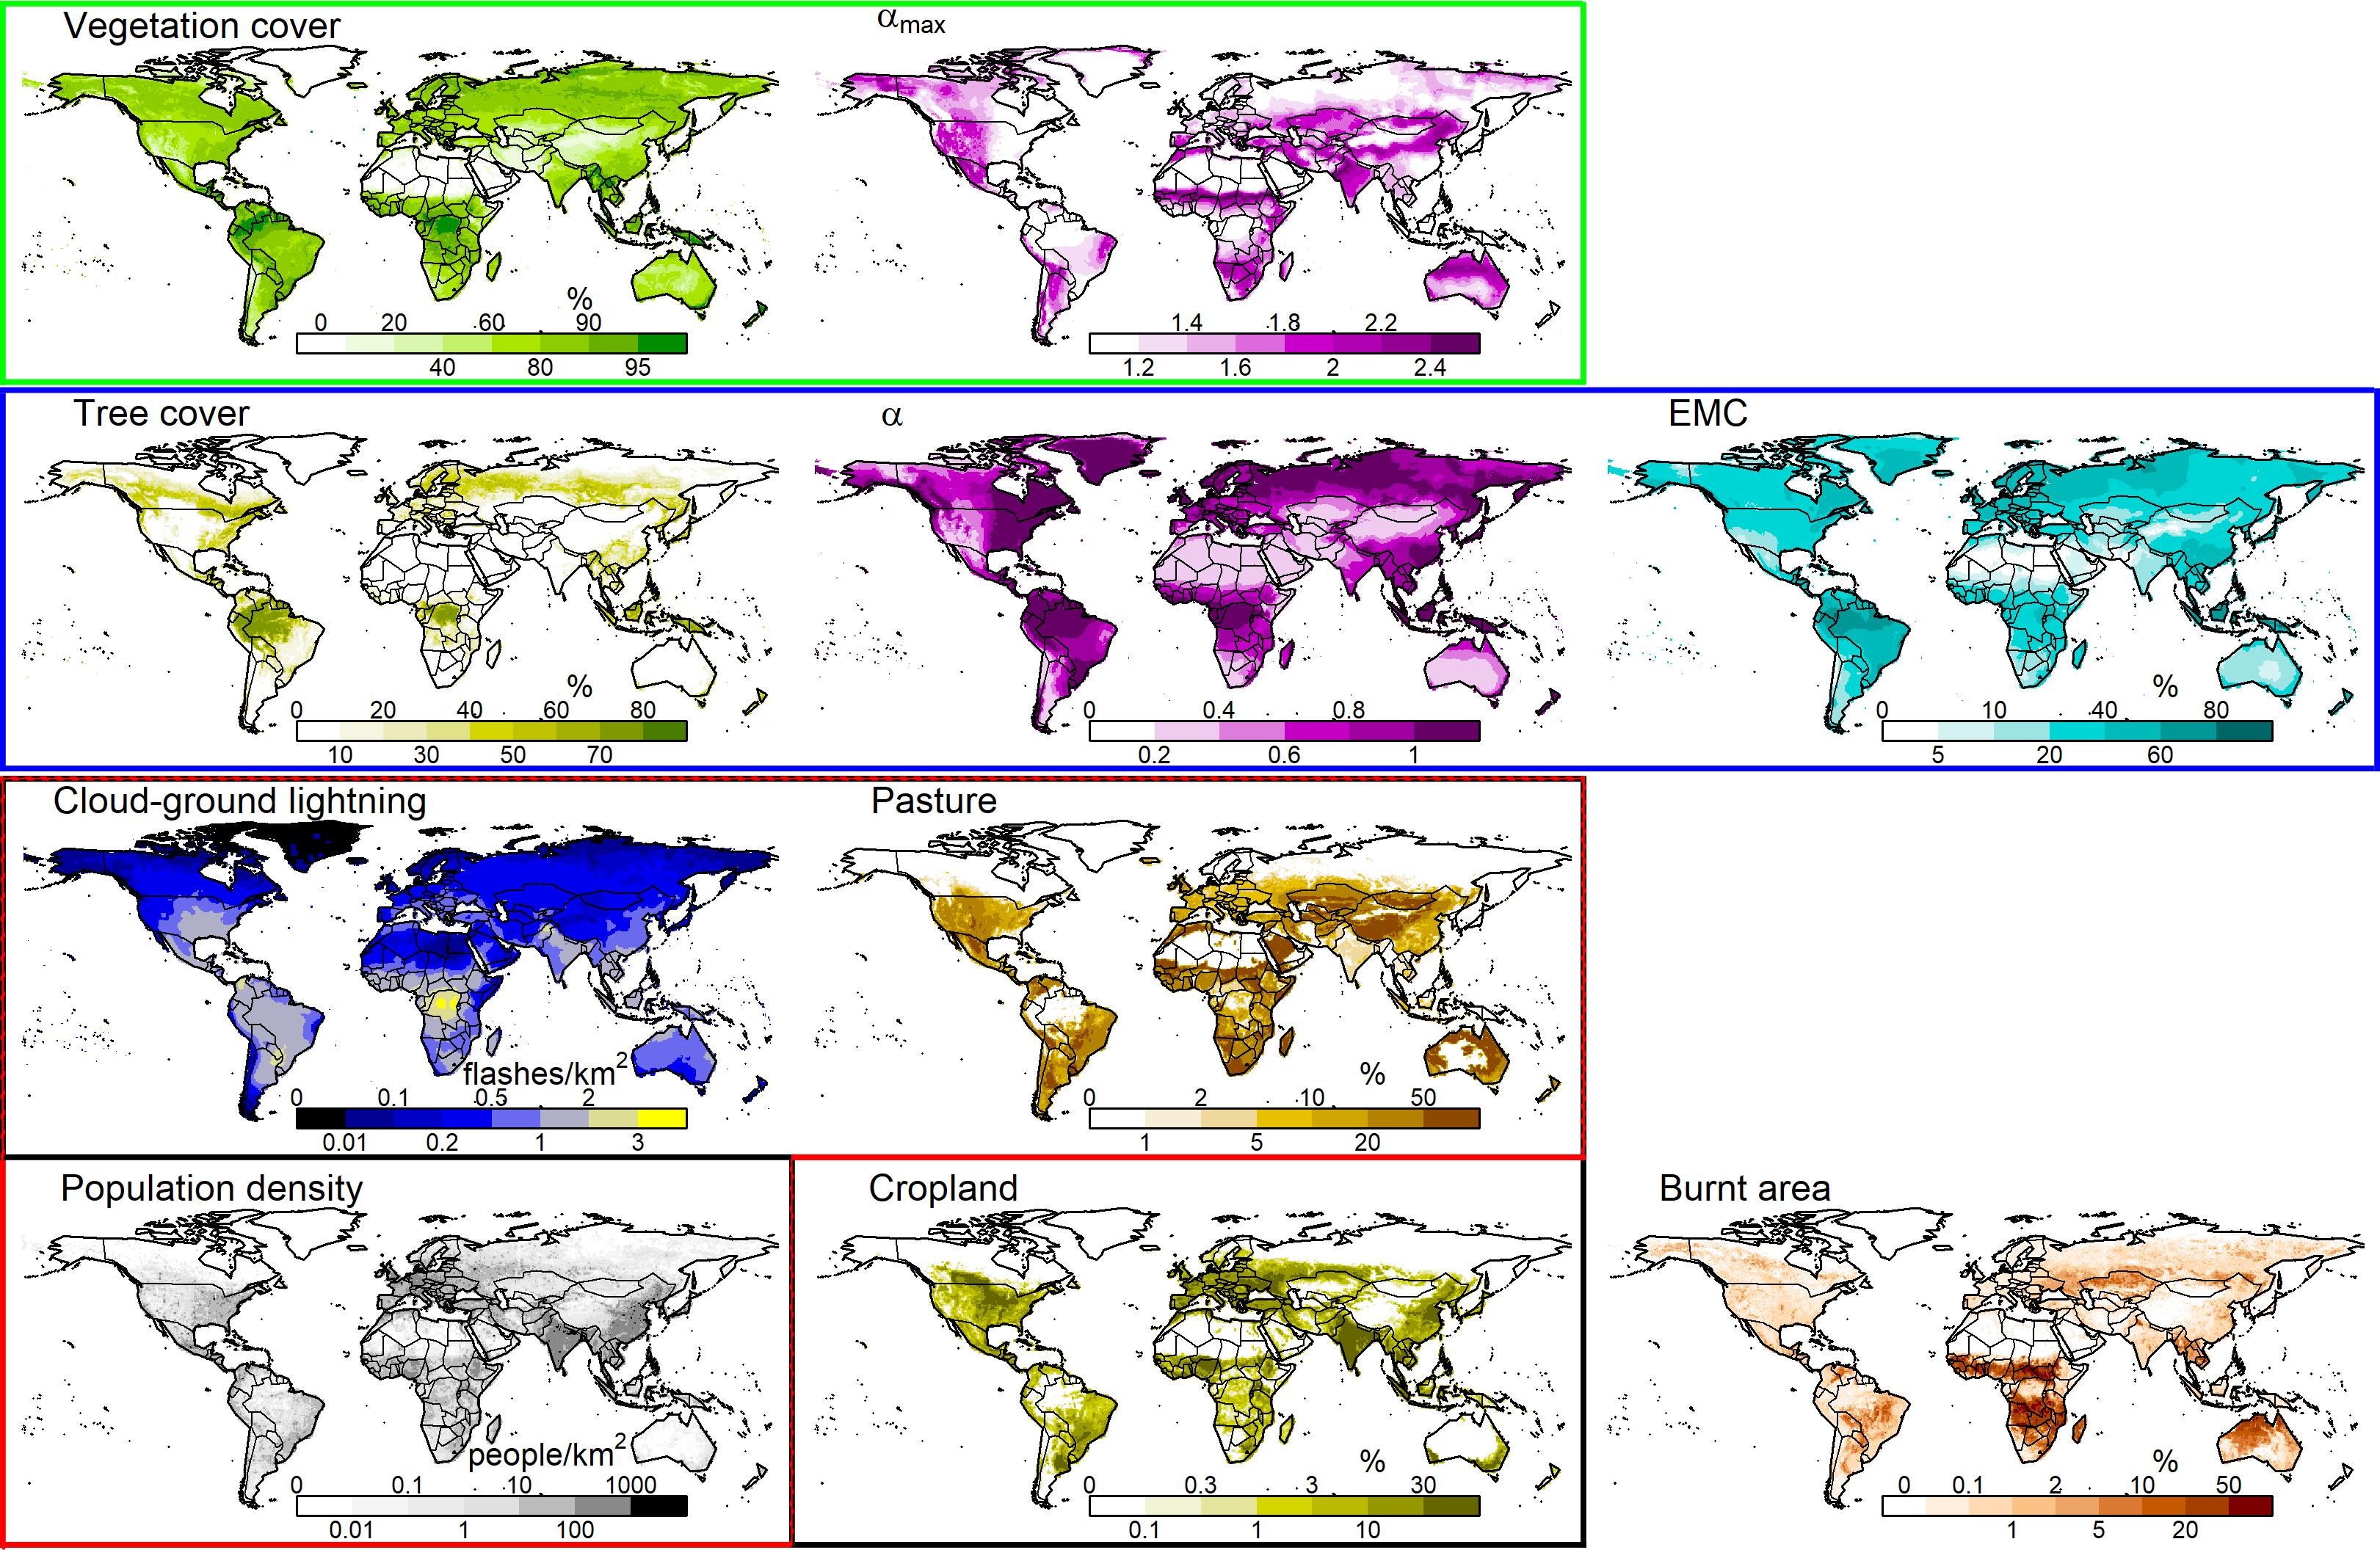
\includegraphics[width=0.67\textwidth]{../figs/inputs_mean.pdf}
  \caption{Monthly means of each framework input \hlr{add units} and GFEDv4.}
  \label{fig:Monthly_mean_ins}
\end{figure}

\begin{figure}[!ht]
  \centering
    \includegraphics[width=0.67\textwidth]{../figs/inputs_fireSeason.pdf}
  \caption{Monthly means during the fire season for each input \hlr{add units} and GFEDv4 training data. ``Fire season'' is defined as the month with heighest burnt area, calculated each year.}
  \label{fig:Season_mean_ins}
\end{figure}

\begin{figure}[!ht]
  \centering
    \includegraphics[width=0.67\textwidth]{../figs/input_correlation.pdf}
  \caption{Input correlations.}
  \label{fig:Corr_ins}
\end{figure}

\subsubsection{Moisture ($\omega$)}

$\omega$ represents mean fractional water content of fuel, and combines contributions from soil (i.e from live fuels - $\alpha$) and atmopshere ($atm$) coupling:

\begin{equation}
    \omega = (\alpha + M \cdot atm) / (1 + M)
\end{equation}

where $M$ is an optimised parameter, representing the relative importance of atmospheric to soil coupling.

\paragraph{Soil-coupled contribution.}
The ratio of actual to potential evaporation \citep[$\alpha$][]{prentice1993simulation}, a measure of available soil water in relation to plant demand, is used to describe fractional water content soil-coupled fuels as per \citet{harrison2010fire, bistinas2014causal}.
$\alpha$ is calculated from CRUTS3.22 monthly mean temperature, cloud cover and precipitation using the STASH model \citep{sykes1996bioclimatic} r-package \citep{rstash}. \hlb{At the moment, elevation, is set to zero and field capacity to 140 - Rhys, I guess this will have to change? Any suggestions for data?}. STASH was spun up by recycling 1950 climate data for 40 years and then run from 1950 to 2010. Simulated $\alpha$ from 2000-2010 used for the rest of the analysis.

\begin{shaded}
\paragraph{Atmosphere-controlled} ($atm$) could be represented using either STASH outputs or by a simple equilibrium moisture content calculation ($m_{mq}$).
\begin{itemize}

\item \textbf{STASH}. The ratio of condensation rate ($Con$) and atmospheric evaportaive demand (i.e $PET$) could be used to calculate ``fuel drying speed'' ($FDS$):

    \begin{equation}
        FDS = \frac{Con}{PET}
    \end{equation}
    here, when $FDS>1$, daily condensation occurs more rapidly than drying, and fuel load mositure will increase, and when $FDS<1$, fuel drys faster then condenstation and fuel moisture will decrease. \\
    \\
    There are a few things to consider here:

    \begin{enumerate}
        \item How should precip be included? Options are to add it to the $Con$ term:

        \begin{equation}
            FDS = \frac{Con + Pr}{PET}
        \end{equation}
        \\
        \\
        or give FDS a maximum value of 1, which is also equivilent to a wetday:

        \begin{equation}
            FDS = WD + (1 - WD) \cdot \min(1, Con/PET)
        \end{equation}
        where $WD$ is fractional wet days
        \\
        \\
        or something else

        \item Is PET being double counted (I couldnt quiet get my head round this bit). If so, there could be a way of combininbg soil and atmopshere:

        \begin{equation}
            \omega_{*} = \frac{AET + C_n}{PET}
        \end{equation}
        \\
        \\
        or maybe

        \begin{equation}
            \omega_{*} = \frac{AET}{PET - C_n}
        \end{equation}
        \\
        \\
        which could also be combined with rainfall:

        \begin{equation}
            \omega = WD + (1 - WD) \cdot min(1, \omega_{*})
        \end{equation}

    \end{enumerate}

    \item $m_{mq}$ is currently used and is calculated from \citep{viney1991review} which combines daily precipitaion ($Pr$) and atmopheric drying potential via temprature ($T$) and relative humidity ($H_r$):

    \begin{equation}
         m_{mq, daily}=
            \begin{cases}
                10 - (T - H_r) / 4 ,& \text{if } Pr\leq 3 \text{mm}\\
                100,              & \text{otherwise}
            \end{cases}
    \end{equation}
    On a monthly timestep, this simplifies to:

    \begin{equation}
         m_{mq}=
            (10 - (T - H_r) / 4) \cdot (1 - WD)
            + 100 \cdot WD
    \end{equation}
    where WD is the monthly fraction of wet days from CRU TS3.22, where a wetday is defined as a day where $Pr > 3mm$. $H_r$ was calculated as the ratio of actual to saturated vapour pressure \hlb{ref??}:

    \begin{equation}
        H_r = 100 \cdot AVP / SVP
    \end{equation}
    monthly $AVP$ is from CRUTS.22. $SVP$ was calculated from mean monthly temperature as per \citet{walter2000asce}

    \begin{equation}
        SVP = 6.11 \cdot 10^{\frac{7.5 \cdot T}{237.5 + T}}
    \end{equation}


    %calculates daily condenstation rates , expressed as the water-equivalent of daily negative net surface radiation:

    %\begin{equation}
    %        C_n = E_{con} \cdot |H^{*}_N| \times 10^3
    %\end{equation}

\end{itemize}

\end{shaded}

\subsubsection{Igntions ($ig$)}

Ignition combines sources from lightning ($L_{ig}$), pasture and the local population.

\begin{equation}
    ig = L_{ig} + P \cdot Pasture + D \cdot Population\text{ }Density
\end{equation}
where P and D are optimized parameters.

\begin{shaded}
    We could also add background igntions:

    \begin{equation}
        ig = 1 + N \cdot L_{ig} + P \cdot Pasture + D \cdot Population\text{ }Density
    \end{equation}
    where N, P and D are opimized paramters describing the contribution of their respective ignition source relative to background igntions.
\end{shaded}


\begin{figure}[!ht]
  \centering
    \includegraphics[width=0.67\textwidth]{../figs/measure_mean.pdf}
  \caption{Monthly means of each control. \hlr{add units?}}
  \label{fig:Monthly_mean_controls}
\end{figure}

\begin{figure}[!ht]
  \centering
    \includegraphics[width=0.67\textwidth]{../figs/measure_fire.pdf}
  \caption{Monthly means of each control during the fire season. \hlr{add units?}}
  \label{fig:Season_mean_controls}
\end{figure}

\paragraph{Lightning}
is calculated from
from the Lightning Imaging Sensor flash count climatology (LIS \cite{christian1999lightning}, http://grip.nsstc.nasa.gov/). \hlb{Are there other products that could be used instead?}
This product contains both cloud-to-ground ($CG$ - available for ignition) and inter-cloud (not available for ignitions) strikes.
$CG$ lighting is calculated using \citet{kelley2014improved}:

\begin{equation}
    L_{ig} = FL * min(1, 0.0408 \cdot FL^{-0.4180})
\end{equation}
where FL is the flash count recorded by LIS over a 0.5 degree cell.

\paragraph{Pasture and population density}
\label{Pasture}
are taken from the HYDE dataset \citep{klein2007mapping}, and are interpolated from a decadal to a monthly timestep.

\subsubsection{Supression ($s$)}

Suppression combines urban and cropland area and population density

\begin{equation}
    s = urban + C \cdot Crop + H \cdot Population\text{ }Density
    \label{equ:Supression}
\end{equation}

where $C$ and $H$ are optimised parameters.

\textbf{Urban} and \textbf{cropland} areas are taken from HYDE and processed as per pasture and population desnity (section ~\ref{Pasture})


\begin{figure}[!ht]
\colorlet{shadecolor}{Mycolor3}
\begin{shaded}
  \centering
    \includegraphics[width=0.67\textwidth]{../figs/limitation_lines.png}

  \caption{Limitation contribution for each control.}
  \label{fig:lim_lines}
\end{shaded}
\colorlet{shadecolor}{Mycolor2}

\end{figure}


\begin{table}[]
\centering
\caption{Optimized paramters obviosuly, to be filled in.}
\label{tab:optimize}
\begin{tabular}{llll}
\hline
\multicolumn{2}{c}{\textbf{Parameter}} & \multicolumn{1}{c}{\textbf{Bound}} & \multicolumn{1}{c}{\textbf{Value}} \\ \hline
\multirow{2}{*}{Fuel}             & $k_{w}$         &                                    &                                    \\
                                  & $x_{0,w}$       &                                    &                                    \\ \hline
\multirow{3}{*}{Moisture}         & $k_{\omega}$    &                                    &                                    \\
                                  & $x_{0, \omega}$ &                                    &                                    \\
                                  & $M$             &                                    &                                    \\ \hline
\multirow{4}{*}{Igntions}         & $k_{ig}$        &                                    &                                    \\
                                  & $x_{0, ig}$     &                                    &                                    \\
                                  & $P$             &                                    &                                    \\
                                  & $D$             &                                    &                                    \\ \hline
\multirow{4}{*}{Human Supression} & $k_{s}$         &                                    &                                    \\
                                  & $x_{0, s}$      &                                    &                                    \\
                                  & $C$             &                                    &                                    \\
                                  & $H$             &                                    &                                    \\ \hline
\end{tabular}
\end{table}

\subsection{Optimization}

\begin{shaded}
    The framework is optimised against GFED4s observations \citep{Giglio2013}  using normalised least squares in R \citep{rstats}.  This is likely to change, though, so I won't describe it anymore for the moment. GFED4s was re-gridded from 0.25 to a 0.5$^{\circ}$ resolution using ``resample'' in the raster r-package \citep{rraster}.
\end{shaded}

\begin{figure}[!ht]
  \centering
    \includegraphics[width=0.67\textwidth]{../figs/ind_limiataionsaa.pdf}
  \caption{Annual average limitation of each control.}
  \label{fig:Annual_average_con}
\end{figure}

\begin{figure}[!ht]
  \centering
    \includegraphics[width=0.67\textwidth]{../figs/ind_limiataionsfs.pdf}
  \caption{Fire season average limitiation of each control.}
  \label{fig:Season_con}
\end{figure}

Optimization is performed on equation ~\ref{equ:LimFIRE} to ~\ref{equ:LimFIRE.x}, 4, 15, 16 and 18 % un-hardcode equations numbers
(figure ~\ref{fig:lim_lines}). Each control optimizes two parameters associated with it's maximum expected burnt area (equations ~\ref{equ:fx} and ~\ref{equ:LimFIRE.x}, see figure ~\ref{fig:Logistic_fun}).
Parameters relating different fuel moisture, ignition and suppression sources are also optimized (see table ~\ref{tab:optimize})


\begin{figure}[!ht]
  \centering
    \includegraphics[width=0.67\textwidth]{../figs/ind_limiataionsaa.pdf}
  \caption{Annual average limitation of each control.}
  \label{fig:Annual_average_con}
\end{figure}

\begin{figure}[!ht]
  \centering
    \includegraphics[width=0.67\textwidth]{../figs/ind_limiataionsfs.pdf}
  \caption{Fire season average limitiation of each control.}
  \label{fig:Season_con}
\end{figure}

\begin{figure}[!ht]
\colorlet{shadecolor}{Mycolor3}
\begin{shaded}
  \centering
    \includegraphics[width=0.9\textwidth]{../figs/gfedComparison.png}
  \caption{Benchmark comparisons against GFED4s \citep{Giglio2013}.}
  \label{fig:benchmark}
\end{shaded}
\colorlet{shadecolor}{Mycolor2}
\end{figure}

\subsection{Benchmarking}
\begin{shaded}
To assess performance of reconstructed burnt area, we'll probably use NME to compare reconstructed fire from the framework with GFED (figure ~\ref{fig:benchmark}) for annual average, seasonal and inter-annual comparisons \citep{kelley2013comprehensive} as recommended by fireMIP \citet{gmd-2016-237, hantson2016status}, and maybe McFaddens $R^{2}$ as per \citep{bistinas2014causal}. Annual average NME comparison comes out at 0.46, which is better than benchmarking null models described in \citet{kelley2013comprehensive}, and outperforms coupled vegetation-fire models contributing to fireMIP \citep{hantson2016status}, although this is to be expected as the framework is driven by, and optimised to, observations \citep{kelley2013comprehensive}.

\end{shaded}

\subsection{Analysis}

\begin{figure}[!ht]
\colorlet{shadecolor}{Mycolor3}
\begin{shaded}
  \centering
    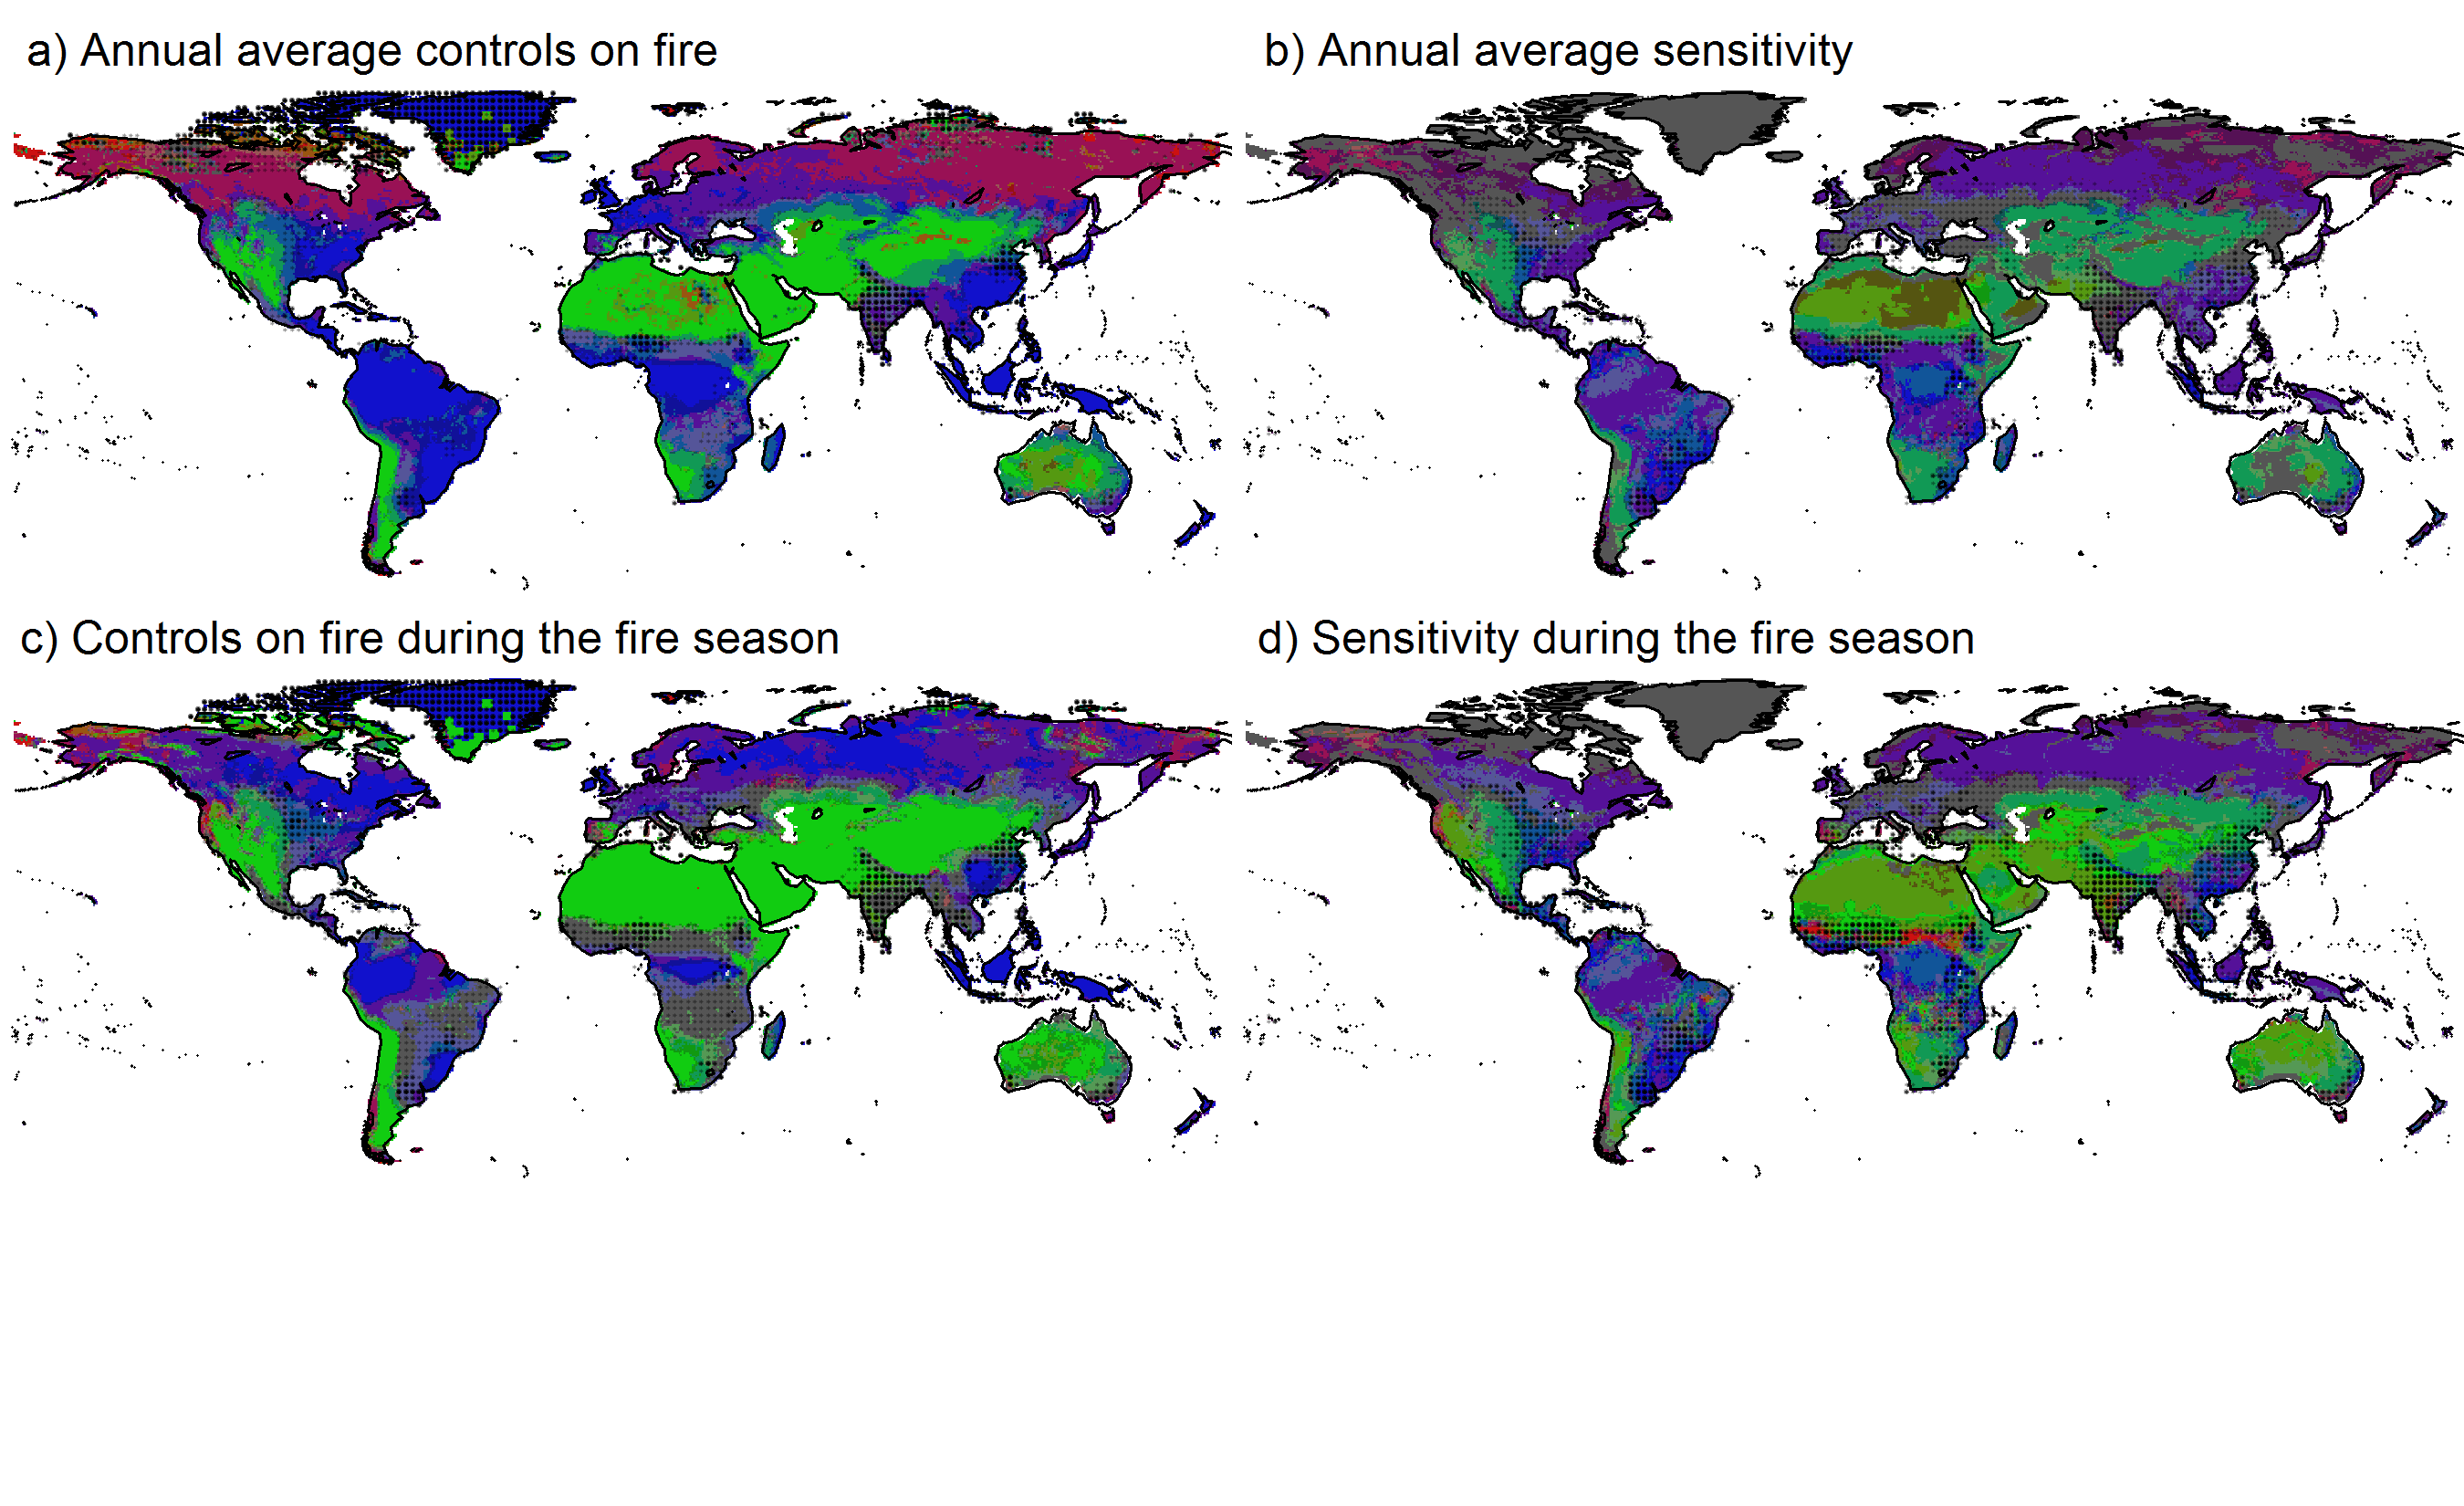
\includegraphics[width=0.9\textwidth]{../figs/limitation_map.png}

  \caption{Limitation and sensitivity.}
  \label{fig:lim_sen_maps}
\end{shaded}
\colorlet{shadecolor}{Mycolor2}
\end{figure}

\subsubsection{Limitation}

The relative importance of each controls was assessed as:

\begin{equation}
    \bar{L_{i, X}} = \frac{L_{i, X}}{\sum_{j} L_{j, X}}
\end{equation}
where $L_{i, X} = 1 - F_{i,X}$ is the individual contribution of each control $i$ for conditions $X$. By definition, $\sum_{i} \bar{L_{i,X}} = 1$, for each location (figures ~\ref{fig:lim_sen_maps} and ~\ref{fig:agu_plot}).


\begin{figure}[!ht]
  \centering
    \includegraphics[width=0.75\textwidth]{../figs/aguplot_Kelleyetal.png}

  \caption{AGU plot.}
  \label{fig:agu_plot}
\end{figure}


\begin{figure}[!ht]
  \centering
    \includegraphics[width=0.67\textwidth]{../figs/moisture_change_for_Amazon_tipping_point.png}

  \caption{Required change in \% fuel moisture content to induce savanna-level fire in the Amazon.}
  \label{fig:amazon}
\end{figure}

\subsubsection{Sensitivity}


\begin{shaded}
    There are two ways I can think of that we could assess sensitivity to each control. We could compare the gradient of each control around the cells current conditions (figure ~\ref{fig:lim_sen_maps}). Alternatively, we could calculate the required change in each control to induce a ``significant'' change in fire regime. The first would be a nice way of classifying different locations, along the same lines as limitations (i.e, Australian Tropical Savanna is xx \% sensitive to changes in fuel load, and yy \% to moisture - see e.g. figure ~\ref{fig:lim_sen_maps}). The second would be harder to normalise across controls, but might be easier to relate to actual changes in climate (i.e, xx $^{\circ}$ increase in temperature would increase fire to expected levels for Savanna - see e.g. figure ~\ref{fig:amazon}; increase in yy \% of agricultural land would reduce fire in non-agricultural land to that expected for forests etc)

\paragraph{options 1}

\begin{equation}
    \bar{\partial L_{i, x}} = \frac{\partial L_{i, x} \cdot \Pi_{j} L_{j, x}}{L_{i, x}}
\end{equation}

where $\partial L_{i, x}$ is the gradient of $L_{i, x}$ relative to the maximum possible gradient of $L_{i}$, occuring when $x = x_{0}$ i.e:

\begin{equation}
    \partial l_{i, x} = \frac{\partial l_{i, x} / \partial X}
                             {\partial l_{i, x_{0}} / \partial x}
\end{equation}

\paragraph{options 2}
for measuring sensitivity is to calculate the change required for a control to alter burnt area enough to induce major alterations in i.e vegetation cover.
For example, assessing amazon risk of fire-induced tipping point. Holding the contribution of ignition, fuel load and land use constant, we could calculate the change in moisture needed to increase burnt area to the level expected for Savanna (roughly 1\% in South America according to \cite{lehmann2011deciphering}).
It would be easy to work out a required change in climate variables (humidity, temperature, ET etc, or any combination of these) required to hit this 'fire tipping point' (figure ~\ref{fig:amazon}).

\end{shaded}
%\pagebreak
\section{Some other results}
\begin{figure}[!ht]
\colorlet{shadecolor}{Mycolor3}
\begin{shaded}
  \centering
    \includegraphics[width=0.8\textwidth]{../figs/HumanImpactMap_small.png}

  \caption{Human impact on burnt area.
            a) Increases in burnt area from human induced fire starts.
            b) Changes in burnt area from human fire starts and suppression.}
    \label{fig:human_impact}
\end{shaded}
\colorlet{shadecolor}{Mycolor2}
\end{figure}

\begin{figure}
\colorlet{shadecolor}{Mycolor3}
\begin{shaded}
  \centering
    \includegraphics[width=0.67\textwidth]{../figs/cropland_noCrop_impact.png}

  \caption{The impact of cropland on burnt area in non-cropland within the same grid cell.}
\end{shaded}
\colorlet{shadecolor}{Mycolor2}
\end{figure}

